\section{Evolução dos materiais}
\subsection*{Idade da Pedra}
Materiais mais comuns: Polímeros (madeiram peles e fibras);Cerâmicos (Pedra)
\subsection*{Idade da Argila}
Materiais mais comuns: 
\subsection*{Idade do Cobre}
Materiais mais comuns: 
\subsection*{Idade do Bronze}
Materiais mais comuns: 
\subsection*{Idade do Ferro}
Materiais mais comuns: 
\section{Sociedade e Materiais}
Aumento significativo de tipos de materiais com o desenvolvimento industrial $\rhd$ Melhoria nos métodos de extração e produção \& Alterações nos materiais para formação de novos materiais (materiais avançados, compósitos)
\section{Classificação dos Materiais}
\subsection*{Metais}
Combinação de elementos metálicos, sendo possível a presença de não-metálicos (ex: aço-carbono).Algumas propriedades relacionadas à presença de elétrons livres (ex: bons condutores de calor e eletricidade).Resistentes e deformáveis: extenso uso em aplicações estruturais.
Suscetível a corrosão.

Possui boa condutividade térmica e elétrica.
\subsection*{Cerâmicos}
ligações de metais e não-metais. Isolantes térmicos e elétricos. Podem ser resistentes a altas temperaturas e a ambientes agressivos. Ex: óxidos, nitretos, carbetos.
Resistentes a corrosão.

Possui boa condutividade térmica e variada condutividade elétrica.
\subsection*{Polímeros}
polímeros:compostos orgânicos. Baixa densidade; altamente deformáveis. (C, H e não-metálicos)
Degrada com solventes, altas temperaturas.

Possui baixa condutividade térmica e elétrica.
\subsection*{Compósitos}
Compósitos: dois ou mais tipos de materiais unidos de forma a produzir um material com características específicas. Projetados para apresentar uma combinação das melhores características de cada um dos componentes.

\subsection*{Materiais avançados}
Usoemaplicaçõesde ponta(altatecnologia). Nãonecessariamentesãonovosmateriais. Podemser tradicionais, com otimizaçãodas propriedades.

\begin{itemize}
		
	\setlength{\parskip}{0pt}
	\setlength{\itemsep}{0pt plus 1pt}
	
\item Alto desempenho
\item Baixo peso e alta resistência
\item Resistência a diversas condições de serviço
\item Ambientalmente corretos
\item Facilmente recicláveis
\end{itemize}
Ex: polímero reforçado com fibra de vidro usado como armadura para estruturas em concreto armado


\section{Classificação dos Materiais}

\subsection*{Qaunto a Estrutura}

\begin{itemize}
		
	\setlength{\parskip}{0pt}
	\setlength{\itemsep}{0pt plus 1pt}
	
	\item Ligações atômicas
	
	\begin{itemize}
			
		\setlength{\parskip}{0pt}
		\setlength{\itemsep}{0pt plus 1pt}
		
		\item Metálica
		\item covalente
		\item iônica
	\end{itemize}

	\item Tipo de Estrutura
	\begin{itemize}
			
		\setlength{\parskip}{0pt}
		\setlength{\itemsep}{0pt plus 1pt}
		
		\item Amorfa
		\item Cristalina
		\item Molecular
	\end{itemize}
\end{itemize}


\subsection*{Propriedades Mecânicas}
\begin{itemize}
		
	\setlength{\parskip}{0pt}
	\setlength{\itemsep}{0pt plus 1pt}
	
	\item dutilidade
	\item elasticidades
	\item dureza
	\item tenacidade
\end{itemize}

\subsection*{Propriedades Químicas e Físicas}
\begin{itemize}
		
	\setlength{\parskip}{0pt}
	\setlength{\itemsep}{0pt plus 1pt}
	
\item	ponto de fusão
\item	calor específico
\item	condutividade (térmica e elétrica)
\item 	Propriedades magnéticas
\item 	Propriedades ópticas
\item 	Iteração com o ambiente: oxidação 
\end{itemize}

\subsection*{Modificação das Propriedades}
\begin{itemize}
		
	\setlength{\parskip}{0pt}
	\setlength{\itemsep}{0pt plus 1pt}
	
	\item Tratamentos térmicos
	\item tratamento de superfície
	\item Tratamentos mecânicos
\end{itemize}


\section{COMPOSIÇÃO QUÍMICA x PROPRIEDADES FÍSICAS}
Exemplo 1: alteração de cor de um mesmo mineral

CORÍNDON:mineral à base de óxido de alumínio (Al2O3)
Chama-se safira qualquer variedade de corindon, de qualidade gemológica, que não seja vermelha (rubi)

Exemplo 2: Alteração da compatibilidade química com o meio ambiente.
Aço patinável (CORTEN): aço com adição de cobre que forma uma pátina, reduzindo o processo corrosivo. Muito usado na construção civil.



\section{ESTRUTURA CRISTALINA x PROPRIEDADES FÍSICAS}
CaCO3

Mármore (calcita -romboédrico)

Conchas (aragonita -ortorrômbico)

\section{TIPO DE LIGAÇÃO QUÍMICA x PROPRIEDADES FÍSICAS}

O tipo de ligação iônica está intimamente ligada com as características físico-química dos materiais.

Temos que:
\subsection*{Ligações Metálicas}
Favorecem a condutividade térmica e elétrica

\subsection*{Ligações Covalentes}
Aparecem em matérias com características isolantes. 


\section{Materiais de Construção}

\subsection*{Escolha do Material}

Etapas básicas

\begin{itemize}
	
\setlength{\parskip}{0pt}
\setlength{\itemsep}{0pt plus 1pt}

\item relacionar experiências prévias para o serviço em questão
\item relacionar e colocar em ordem de prioridade todos os parâmetros que podem influenciar na escolha
\item estabelecer as características que se deseja para o material ideal ao serviço
\item realizar testes, comparando os materiais que possam ser usados otimizando o custo total.

\end{itemize}

Definição da categoria do material: metal, cerâmico, polímero ou compósito

\subsection*{Como selecionar um material?}

Condições operacionais
\begin{itemize}
	
	\setlength{\parskip}{0pt}
	\setlength{\itemsep}{0pt plus 1pt}
	
\item Custo/benefício (indústria de massa ou de grande exigência tecnológica?)
\item Propriedades requeridas
\item Degradação no meio
\item Solicitação mecânica
\item Resistência/peso
\end{itemize}

\subsection*{Quais fatores influenciam na escolha dos materiais para determinado serviço ou aplicação industrial?}

\begin{itemize}
	\item Propriedades físicas e químicas 
	\item Características operacionais
	\item Fabricação, disponibilidade e custo
	
\end{itemize}


\section{Propriedades físicas e químicas}

\subsection*{Propriedades mecânicas}
Limites de escoamento e de resistência, dutilidade, resistência à fadiga e fluência, temperatura de transição dúctil-frágil, módulo de elasticidade.

\subsection{Outras propriedades físicas}
densidade, calor específico,expansão térmica,condutividade,propriedades magnéticas e elétricas.


\subsection*{Propriedades químicas}
oxidação, flamabilidade, toxicidade.

\section{Características operacionais}

\subsection*{temperatura}
\subsection*{natureza dos fluidos em contato com material}
(composição química, concentração, pH, caráter oxidante ou redutor, presença de contaminantes, pressão, velocidade do fluido, flamabilidade, toxidez). Necessário avaliar alterações em cada um destes fatores ao longo do tempo de serviço.

\subsection*{presença de resíduos oriundos de processos corrosivos}
ex: alguns materiais como o chumbo são resistentes à corrosão porém geram resíduos tóxidos, limitando seu uso.

\section{Fabricação,disponibilidade e custo}


\subsection*{Fatores críticos na seleção:} facilidade de fabricação e forma de apresentação. Ex:espessura de chapas e formato(tubos ou tarugos)
Custo/benefício: custo direto do material, tempo de vida útil e custos indiretos (paradas para reparos ou reposição dos equipamentos).
Tempo de vida útil compatível com tempo previsto de operação.
Relação direta com segurança (acidentes e falhas)
Furos em tubulações.
Aço inox 304 no lugar de aço-C.
Aço-carbono disponível em inúmeras formas de fabricação.


\section{Estrutura Cristalina}

\subsection*{Material Amorfo X Cristalino}
O material CRISTALINO possui arranjo mais uniforme e as moléculas está direcionadas de forma a apresentarem um densidade molecular maior. 

O material AMORFO possui suas moléculas dispostas de forma mais aleatória e a densidade molecular dessa região é menor.


\subsection*{CRISTALINIDADE} Arranjo interno ordenado das partículas segundo um modelo tridimensional, característico do estado sólido. Em muitos corpos a cristalinidade é evidenciada por faces e simetria externa, indicando um arranjo ordenado dos átomos. Exames em raios X(1912) estudo de substâncias inorgânicas.

\subsection*{CRISTALOGRAFIA} Estudo dos corpos sólidos que possuem estrutura cristalina e das leis que governam seu crescimento, forma externa e interna. É instrumento fundamental na química, física, metalurgia e no estudos das cerâmicas, refratários, semicondutores, gemas sintéticas, etc.


\subsection*{CÉLULAS UNITÁRIAS} para a maioria dos cristais, as células unitárias podem ser representadas por geometrias específicas. Mais do que uma célula unitária pode ser escolhida para representar o cristal. Geralmente, escolhe-se a que apresenta o maior grau de simetria geométrica.



\subsection*{SISTEMAS CRISTALINOS} Qualquer empacotamento atômico deverá se encaixar em um dos sete principais tipos de cristais, que estão intimamente associados com o modo pelo qual o espaço pode ser dividido em volumes iguais, pela interseção de superfícies planas.
Existem diferentes estruturas cristalinas possíveis. É conveniente dividi-las em grupos de acordo com as configurações das células unitárias e/ou os arranjos atômicos. Para criar todos os tipos de redes são necessários sete tipos distintos de células cristalinas.


\section{Células unitárias e Sistemas cristalinos}

Parâmetros de rede cristalina:
\begin{itemize}
	\item a,b,c - comprimentos dos lados do paralelepípedo
	\item $ \alpha$, $\beta$, $\gamma $ - ângulos entre os eixos
\end{itemize}

$\gamma $





Com base nestes parâmetros de rede, tem-se que existem 7 diferentes combinações possíveis entre a,b,c e $\alpha, \beta, \gamma $ cada um representando um sistema cristalino.


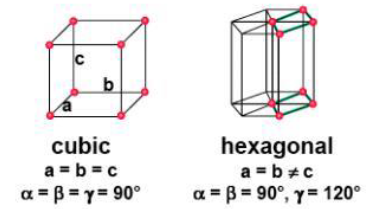
\includegraphics[scale=0.5,trim={0 0 0 0}]{figures/crist1}
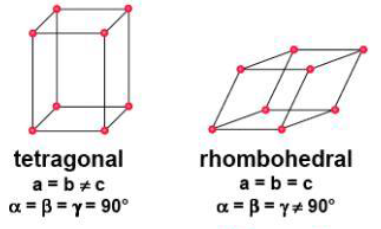
\includegraphics[scale=0.5,trim={0 0 0 0}]{figures/crist2}
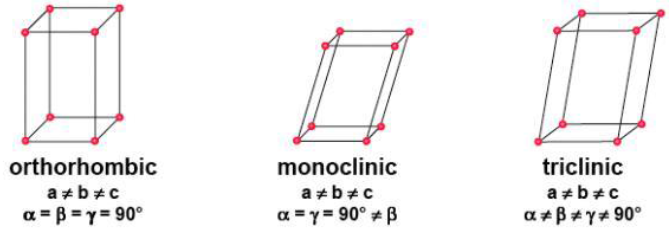
\includegraphics[scale=0.3,trim={0 0 0 0}]{figures/crist3}


O maior grau de simetria aparece no sistema cúbico e o menor grau é visto no sistema triclínico.

\subsection*{Variações na célula unitária básica}

As possíveis redes podem ser descritas por 14 células unitárias (A.J. Bravais).
Em algumas células unitárias existem alguns tipos básicos: simples, de corpo centrado e de faces centradas.
 
 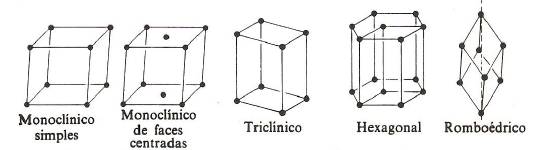
\includegraphics[scale=0.5,trim={0 0 0 0}]{figures/var1}
 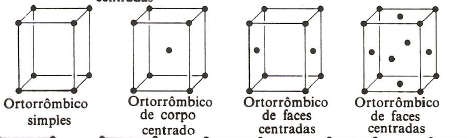
\includegraphics[scale=0.45,trim={0 0 0 0}]{figures/var2}
 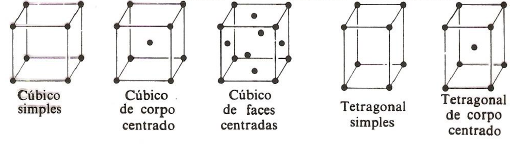
\includegraphics[scale=0.5,trim={0 0 0 0}]{figures/var3}



Agora eu posso colocar mais variedades e salvar direto no meu git

Ai eu faço todas alterações e rodo o programa bat


 
%\subsection*{Aussage}
%Eine Aussage ist ein Satz, der entweder wahr oder falsch ist, also nie beides zugleich.
%Wahre Aussagen haben den Wahrheitswert $w$ und falsche Aussagen den
%Wahrheitswert $f$.
%\subsection*{Belegung von Variablen}
%Sei $\mathcal{A}_B(F) = f$.
%Dann ist stets $\mathcal{A}_B(F\Rightarrow G) = w$
%\subsection*{Formelbeweis über Belegung}
%Wenn $F \wedge G$ eine Tautologie ist, dann (und nur dann) ist $F$ eine Tautologie und $G$ auch.
%Hinweis: In dem Lemma stecken zwei Teilaussagen, die beide zu beweisen sind:
%1. Wenn $F \wedge G$ eine Tautologie ist, dann ist $F$ eine Tautologie und $G$ auch.
%2. Umgekehrt: Sind $F$ und $G$ Tautologien, dann ist auch $F \wedge G$ eine.
%\emph{Beweis.}
%1. Annahme: $F \wedge G$ sei eine Tautologie.
%Dann: Für jede Belegung $B$ wertet $F \wedge G$ zu wahr aus.
%Dann: Das ist nur der Fall, wenn sowohl $F$ als auch $G$ (für jedes $B$) zu wahr auswerten.
%Dann: Für jede Belegung $B$ wertet $F$ zu wahr aus. Und:
%Für jede Belegung $B$ wertet $G$ zu wahr aus.
%Dann: $F$ ist Tautologie und $G$ ist Tautologie.
%2. Annahme: $F$ ist Tautologie und $G$ ist Tautologie.
%Dann: Für jede Belegung $B_1$ wertet $F$ zu wahr aus. Und: Für jede Belegung $B_2$ wertet $G$ zu wahr aus.
%Dann: Für jede Belegung $B$ wertet $F \wedge G$ zu wahr aus.
%Dann: $F \wedge G$ ist eine Tautologie.
%\subsection*{Äquivalenz und Folgerung}
%$p\equiv q$ gilt genau dann, wenn sowohl $p\models q$ als auch $q\models p$ gelten. \emph{Beweis.}
%$p\equiv q$ GDW $p\Leftrightarrow q$ ist Tautologie nach Def. von $\equiv$
%GDW $(p\Rightarrow q) \wedge (q\Rightarrow p)$ ist Tautologie
%GDW $(p\Rightarrow q)$ ist Tautologie und $(q\Rightarrow p)$ ist Tautologie
%GDW $(p\models q)$ gilt und $q\models p$ gilt.
%\subsection*{Substitution}
%Ersetzt man in einer Formel eine beliebige Teilformel $F$ durch eine logisch äquivalente
%Teilformel $F'$, so verändert sich der Wahrheitswerteverlauf der Gesamtformel nicht.
%Man kann Formeln also vereinfachen, indem man Teilformeln durch äquivalente
%(einfachere) Teilformeln ersetzt.
%\subsection*{Universum}
%Die freien Variablen in einer Aussagenform können durch Objekte aus einer als
%Universum bezeichneten Gesamtheit wie $\mathbb{N},\mathbb{R},\mathbb{Z},\mathbb{Q}$ ersetzt werden.
%\subsection*{Tautologien}
%$(p\wedge q)\Rightarrow p$\text{ bzw. }$p\Rightarrow (p\vee q)$\\
%$(q\Rightarrow p)\vee (\neg q\Rightarrow p)$\\
%$(p\Rightarrow q)\Leftrightarrow (\neg p\vee q)$\\
%$(p\Rightarrow q)\Leftrightarrow (\neg q\Rightarrow\neg p)$ \hfill\text{(Kontraposition)}\\
%$(p\wedge (p\Rightarrow q))\Rightarrow q$ \hfill\text{(Modus Ponens)}\\
%$((p\Rightarrow q)\wedge (q\Rightarrow r))\Rightarrow (p\Rightarrow r)$\\
%$((p\Rightarrow q)\wedge (p\Rightarrow r))\Rightarrow (p\Rightarrow (q\wedge r))$\\
%$((p\Rightarrow q)\wedge (q\Rightarrow p))\Leftrightarrow (p\Leftrightarrow q)$
%\subsection*{Nützliche Äquivalenzen}
%Kommutativität:\\
%$(p \wedge q) \equiv (q \wedge p)$\\
%$(p \vee q) \equiv (q \vee p)$\\
%Assoziativität:\\
%$(p \wedge (q \wedge r)) \equiv ((p \wedge q) \wedge r)$\\
%$(p \vee (q \vee r)) \equiv ((p \vee q) \vee r)$\\
%Distributivität:\\
%$(p \wedge (q \vee r)) \equiv ((p \wedge q) \vee (p \wedge r))$\\
%$(p \vee (q \wedge r)) \equiv ((p \vee q) \wedge (p \vee r))$\\
%Idempotenz:\\
%$(p \wedge p) \equiv p$\\
%$(p \vee p) \equiv p$\\
%Doppelnegation:\\
%$\neg (\neg p) \equiv p$\\
%de Morgans Regeln:\\
%$\neg (p \wedge q) \equiv ((\neg p) \vee (\neg q))$\\
%$\neg (p \vee q) \equiv ((\neg p) \wedge (\neg q))$\\
%Definition Implikation:\\
%$(p \Rightarrow q) \equiv (\neg p \vee q)$\\
%Tautologieregeln:\\
%$(p \wedge q) \equiv p$\hfill (falls $q$ eine Tautologie ist)\\
%$(p \vee q) \equiv q$\\
%Kontradiktionsregeln:\\
%$(p \wedge q) \equiv q$\hfill (falls $q$ eine Kontradiktion ist)\\
%$(p \vee q) \equiv p$\\
%Absorptionsregeln:\\
%$(p \wedge (p \vee q)) \equiv p$\\
%$(p \vee (p \wedge q)) \equiv p$\\
%Prinzip vom ausgeschlossenen Dritten:\\
%$p \vee (\neg p) \equiv w$\\\
%Prinzip vom ausgeschlossenen Widerspruch:\\
%$p \wedge (\neg p) \equiv f$
%\subsection*{Äquivalenzen von quant. Aussagen}
%Negationsregeln:\\
%$\neg\forall x:p(x)\equiv\exists x:(\neg p(x))$\\
%$\neg\exists x:p(x)\equiv\forall x:(\neg p(x))$\\
%Ausklammerregeln:\\
%$(\forall x:p(x)\wedge\forall y:q(y))\equiv\forall z:(p(z)\wedge q(z))$\\
%$(\exists x:p(x)\wedge\exists y:q(y))\equiv\exists z:(p(z)\wedge q(z))$\\
%Vertauschungsregeln\\
%$\forall x\forall y:p(x,y)\equiv\forall y\forall x:p(x,y)$\\
%$\exists x\exists y:p(x,y)\equiv\forall y\exists x:p(x,y)$
%\subsection*{Äquivalenzumformung}
%Wir demonstrieren an der Formel $\neg (\neg p \wedge q) \wedge (p \vee q)$, wie man mit Hilfe der
%aufgelisteten logischen Äquivalenzen tatsächlich zu Vereinfachungen kommen kann:\\
%$\phantom{{}\equiv{}} \neg (\neg p \wedge q) \wedge (p \vee q)$\\
%$\equiv (\neg (\neg p) \vee (\neg q)) \wedge (p \vee q)$\hfill de Morgan\\
%$\equiv (p \vee (\neg q)) \wedge (p \vee q)$\hfill Doppelnegation\\
%$\equiv p \vee ((\neg q) \wedge q)$\hfill Distributivtät v.r.n.l.\\
%$\equiv p \vee (q \wedge (\neg q))$\hfill Kommutativtät\\
%$\equiv p \vee f$\hfill Prinzip v. ausgeschl. Widerspruch\\
%$\equiv p$\hfill Kontradiktionsregel
%\subsection*{Quantifizierte Aussagen}
%Sei $p(x)$ eine Aussageform über dem Universum $U$.
%$\exists x : p(x)$ ist wahr genau dann, wenn ein $u$ in $U$ existiert, so dass $p(u)$ wahr ist.
%$\forall x : p(x)$ ist wahr genau dann, wenn $p(u)$ für jedes $u$ aus $U$ wahr ist.
